
This section of the thesis outlines the methodology used for data analysis, cleaning, transformation, feature engineering, and machine learning experiments.
Data-driven methods have the potential to learn all relations in the data, but the size of the dataset limits this.
Therefore, cleaning the data and selecting features containing information relevant to the desired output is essential.
With the system's complexity, identifying relevant features can be challenging.
To address this, we employ data-driven modeling to help identify important features while using feature engineering to incorporate
our understanding of the system and create informative features.

Cleaning data involves removing irrelevant data that could confuse the model, thereby ensuring that the model learns from the most relevant information.
Feature engineering involves incorporating domain knowledge into the model to create features that provide additional information.

We perform data analysis to decide which features to train our models.
This analysis involves understanding the relationships between the different variables in the dataset and identifying which variables
could be helpful in predicting the target variable.
The outcome of the data analysis informs our decisions on which features to use in the models.


\section{Cleaning pointing scan data} \label{sec:cleaning_pt_scan}

When utilizing data-driven modeling for predictive purposes, ensuring that the dataset is clean and informative is crucial.
In this project, various factors may impact the quality of the data, and therefore, we implemented measures to clean the data based on our knowledge of the telescope's operation.
We employed a criteria-based approach and a machine learning classifier to remove pointing scans from the dataset.
During the removal of pointing scans, it is important to strike a balance between removing noise and retaining relevant information.
Outliers in the training data can introduce bias into machine learning models, as these data points may not accurately represent real-world conditions.
Consequently, having outliers in the training data can be more damaging than removing good pointing scans.
Therefore, we have a strict approach when cleaning the data to ensure high-quality datasets for model training.


\subsection{Cleaning criteria}
To eliminate unreliable or unusable scans, we applied criteria informed by the insights of astronomers at APEX.
The following list outlines the criteria used to filter out such scans:
\begin{itemize}
    \item Scans using the HOLO transmitter:
    These scans are aimed at a radio tower and are not realistic data for training an ML model.
    \item Scans using ZEUS2:
    These are highly experimental pointing scans and unreliable.
    \item Scans using CHAMP690: There are very few scans with this instrument.
    \item Scans in January and February of $2022$: The weather is unreliable and there are few scans in this period.
    \item Scans that are tracking tests
    \item Scans after 17.09.2022 since we only have sensory data until this point
\end{itemize}   
After this filtering, there are $5901$ out of $8862$ scans left.
        
\subsection{Pointing scan classifier} 
\subsubsection{Method}
In addition to cleaning the data based on the criteria above, we had to remove the outright bad pointing scans (like \ref{subfig:bad_continuous} \ref{subfig:bad_line}, \ref{subfig:bad_line}).
The scan quality is often obvious when inspecting the data visually, but it is hard to develop suitable measures to identify which scans are good or bad.
Instead, we trained a classifier to predict whether a scan is of good or bad quality.
We used an XGBoost classifier with 13 features as inputs, all of which are present in the pointing scan figures (\ref{fig:line_pointings} and \ref{fig:continueous_pointings}).
The first 12 features are the amplitudes, FWHMs, pointing offsets, and these values' uncertainties.
The last feature is the beamsize of the telescope for the given observing frequency.\\

We had to label a training set by manually looking at pointing scans.
The size of the training set was $369$ samples with $270$ good and $99$ bad scans.
Table \ref{tab:xgb_hyperparameters_clf} shows the hyperparameters and search ranges we used when optimizing this model, along with the resulting best parameter values.
We also used \textit{scale\_pos\_weight} to consider the unbalanced classes, for which the value is the ratio of negative to positive classes (number of bad scans divided by number of good scans).
We split the data into $80\%$ for training and the rest for testing, corresponding to $295$ and $74$ samples for training and testing, respectively.

\begin{table}[H]
    \centering
    \caption{This table presents a list of parameters we sampled during hyperparameter tuning for the pointing scan classifier.
    The table includes names, sampled distributions and corresponding ranges, and parameter values for the best model.}
    \begin{tabular}{lccc}
        \toprule
        Parameter & Sample Distribution & Range & Best Parameter Value\\ \hline
        max depth & Uniform & [$1$, $5$] & $2$\\ 
        n estimators & Uniform & [$1$, $80$] & $53$\\ 
        \bottomrule
    \end{tabular}
    \label{tab:xgb_hyperparameters_clf}
\end{table}

\subsubsection{Results}
The XGBoost classifier performed well with a $97\%$ overall accuracy on the test set.
Figure \ref{fig:pointing_scan_clf} shows the precision-recall curve on the left and the average precision curve on the right.
From the precision-recall curve, it is clear that we can achieve close to $100\%$ precision while still having a high recall.
We select a large threshold such that the classifier removes most bad scans from the training data,
because a bad pointing scan is potentially more harmful for the model than discarding a few good scans.
The average precision curve shows an optimal threshold for maximizing the precision, which is about $80\%$.\\

Using the classifier to further clean the dataset, using prediction threshold $0.8$, we remove another $575$ scans, leaving us with
$5326$ scans for the rest of the analysis.


\begin{figure}[H]
    \centering
    \begin{subfigure}[t]{0.49\textwidth}
        \centering
        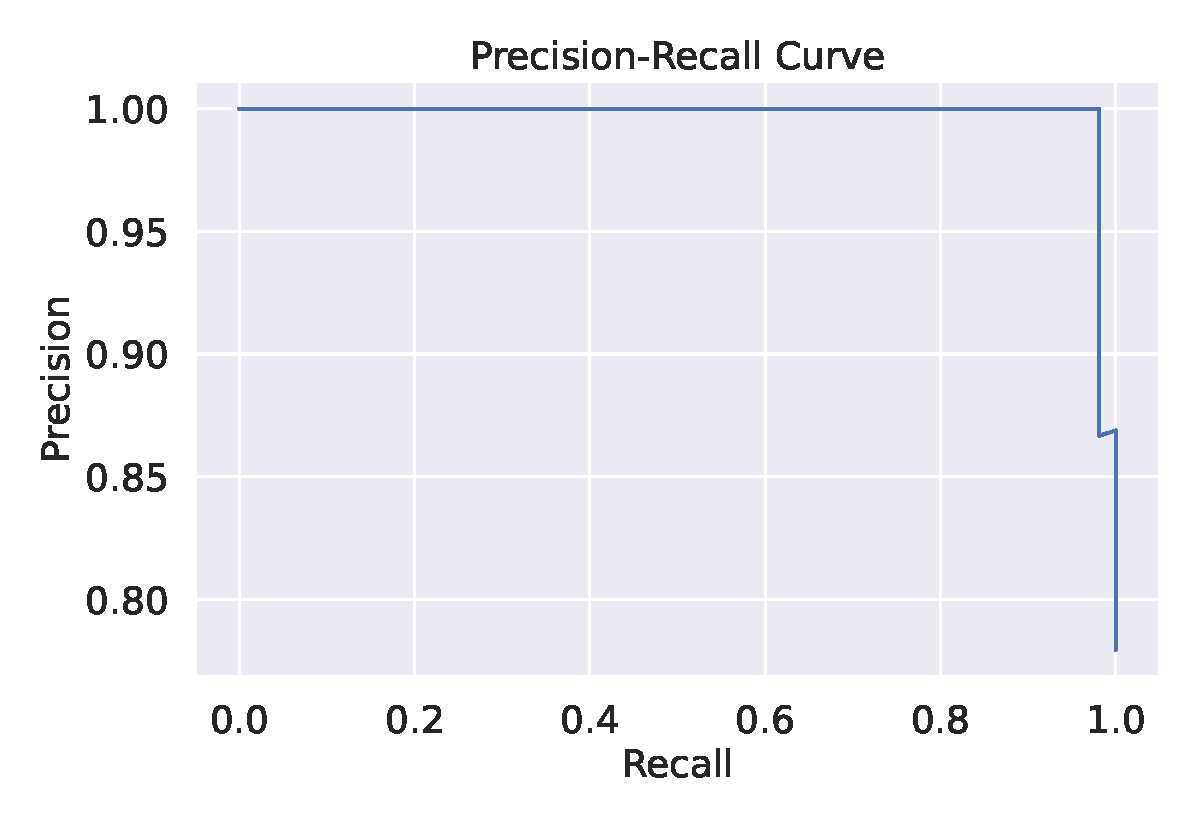
\includegraphics[width=1\textwidth]{Clf/precision_recall_curve_both.pdf}
        \caption{Precision-recall curve on the test set.}
        \label{subfig:pr_curve}
    \end{subfigure}
    \begin{subfigure}[t]{0.49\textwidth}
       \centering
       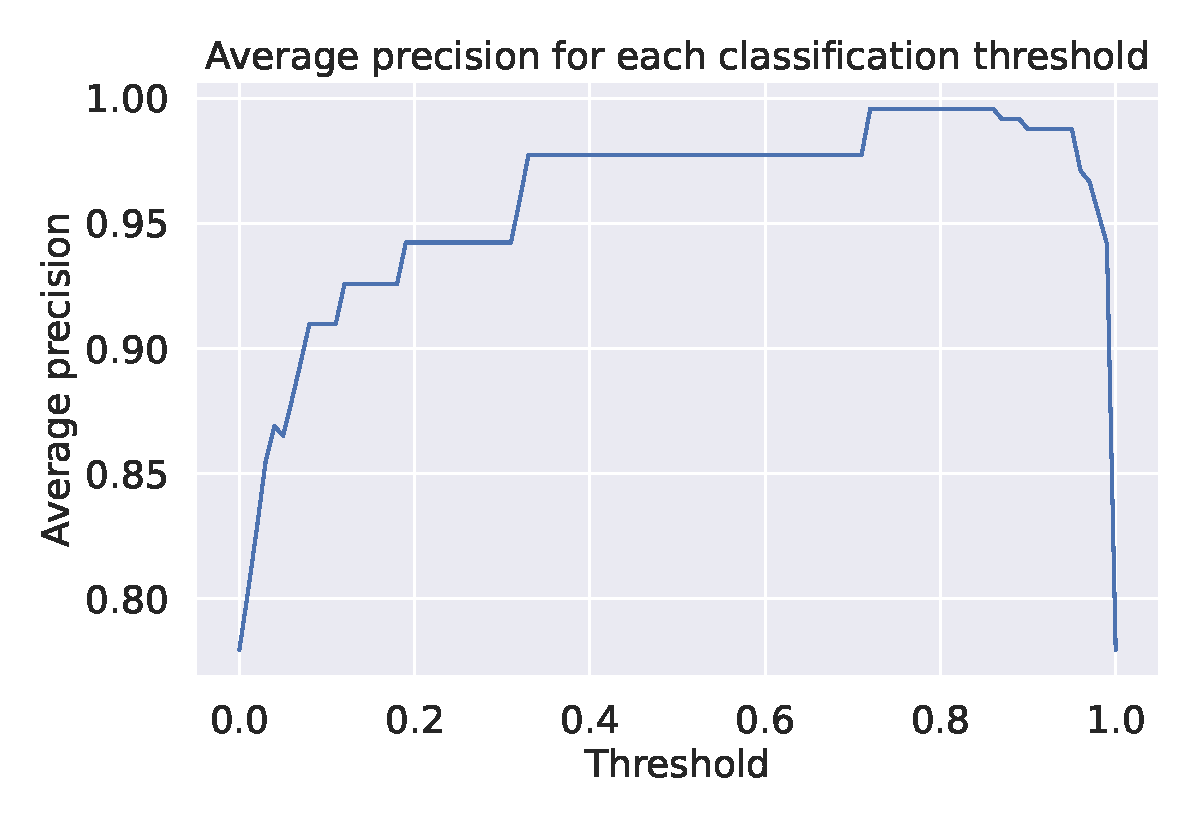
\includegraphics[width=1\textwidth]{Clf/mAP_curve_both.pdf}
       \caption{Average precision for different classification threshold.}
       \label{subfig:map_curve}
    \end{subfigure}
     \caption{Precision-recall and average precision curve for the XGBoost classifier when classifying good and bad pointing scans in the test set.}
     \label{fig:pointing_scan_clf}
\end{figure}



% \\~\\
% \begin{subfigure}[t]{0.49\textwidth}
%     \centering
%     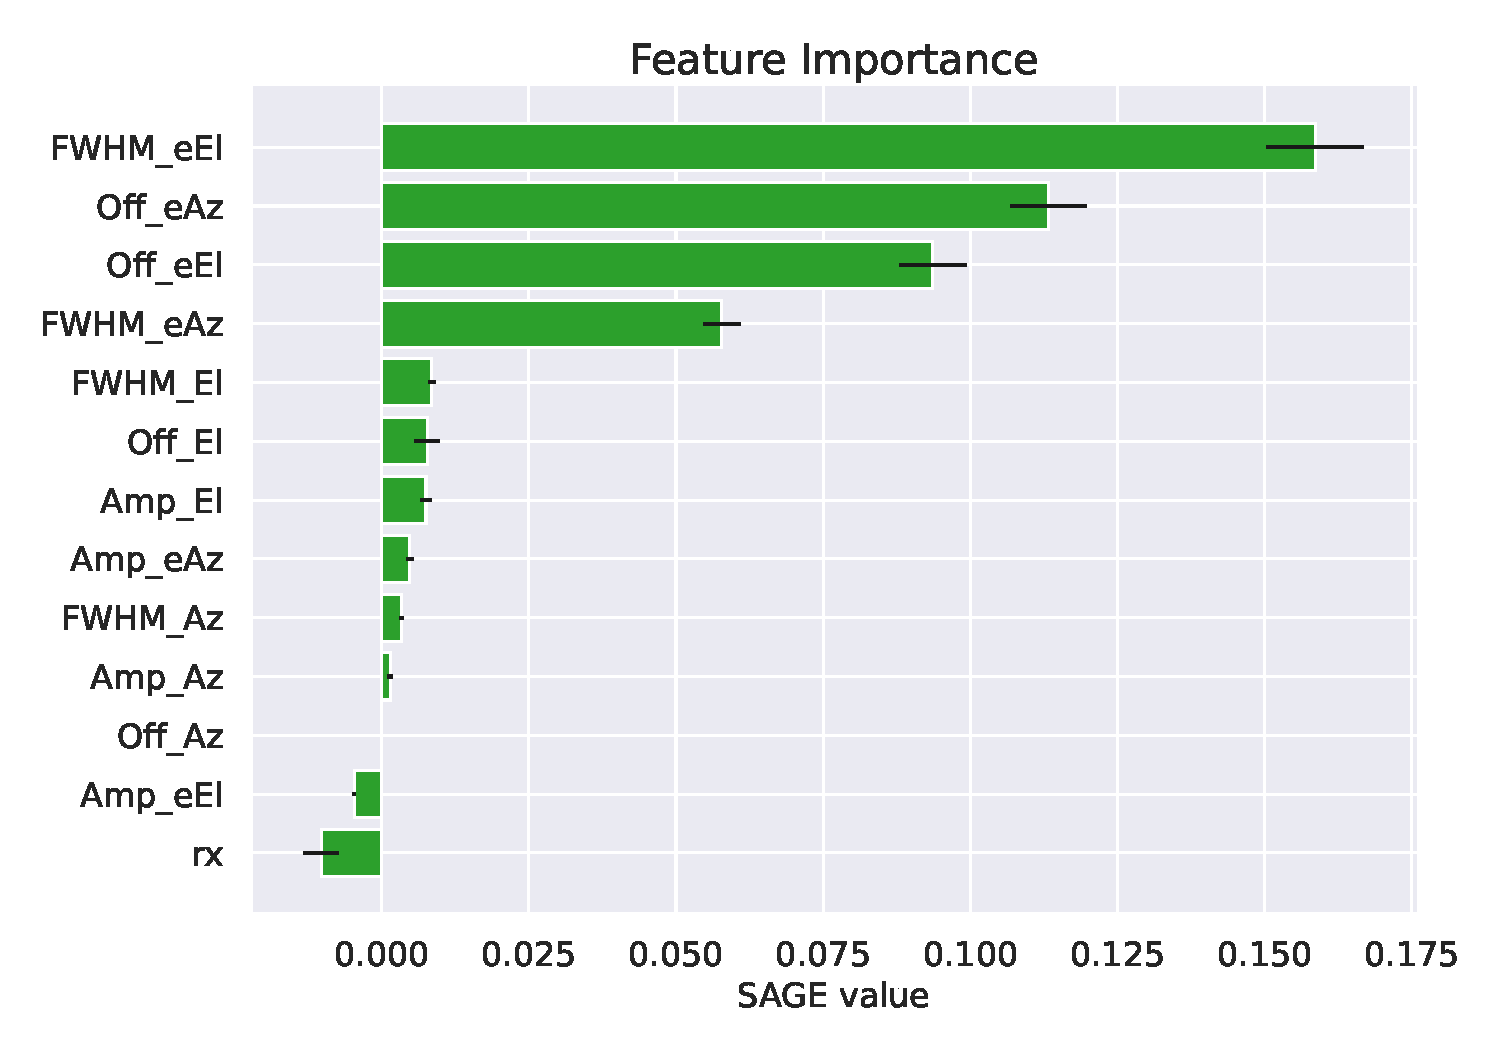
\includegraphics[width=1\textwidth]{Clf/Sage_xgb_clf_rx.pdf}
%     \caption{Average precision for different classification threshold.}
%     \label{subfig:xgb_clf_sage}
% \end{subfigure}
% \begin{figure}[H]
%     \centering
%     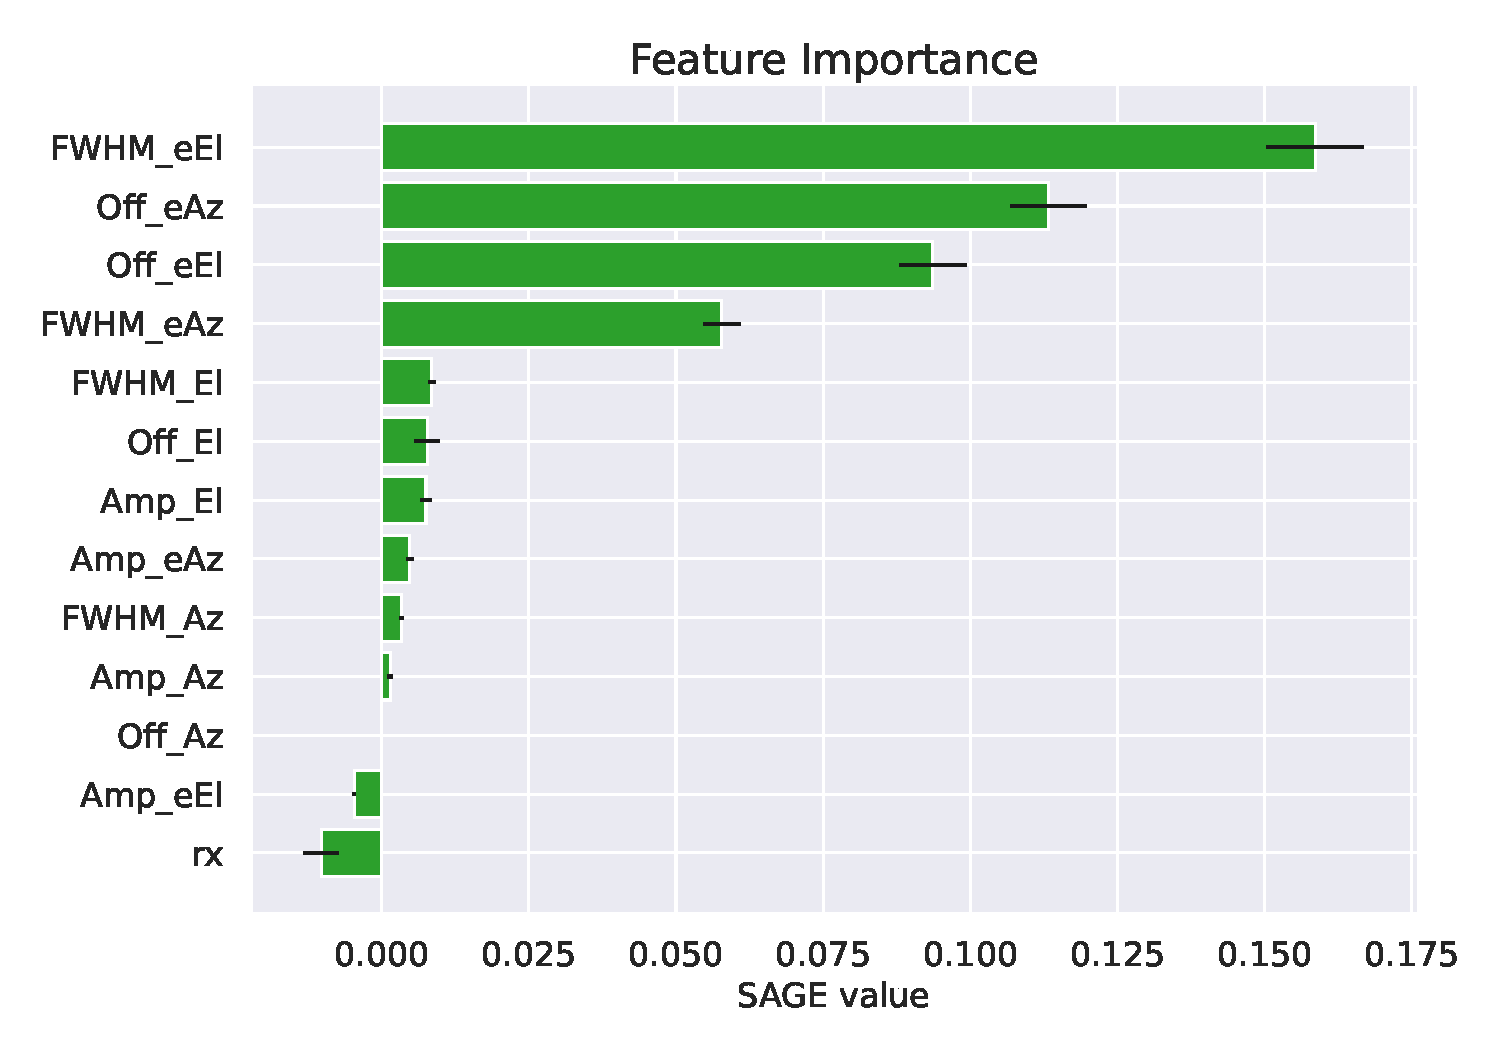
\includegraphics[width=0.98\textwidth]{Clf/Sage_xgb_clf_rx.pdf}
%     \caption{SAGE values for the XGB classifier.}
%     \label{fig:xgb_clf_sage}
% \end{figure}

\section{Scan duration analysis}\label{sec:scan_duration_analysis}
As mentioned in the database section \ref{sec:database}, the scans' timestamps are not the accurate start time of a scan.
The tiltmeter dump files with the flag indicating whether the telescope is idle, preparing to observe, or observing,
is the only accurate data we have when the telescope performs a pointing scan.
Therefore, we need to combine the timestamp of the pointing scan with the flag in the dump files to analyze the duration of scans.

\subsection{Analysis}
First, we convert the different scan flags to numbers.
\textit{IDLE} and \textit{PREPARING} is the set $0$, and \textit{OBSERVING} is set to $1$.
Then we can subtract the previous rows from all rows, resulting in the value $1$ when the scan starts, and $-1$ when it ends.
Table \ref{tab:scan_flag_difference} shows an example of the resulting table.


\begin{table}[H]
    \centering
    \begin{tabular}{cccc}
        \toprule
        Time & Flag & Flag Integer & $\Delta$ \\
        \midrule
        11:21:21 & IDLE & $0$ & $0$ \\
        11:21:22 & PREPARING & $0$ & $0$ \\
        11:21:23 & OBSERVING & $1$ & $1$ \\
        11:21:24 & OBSERVING & $1$ & $0$ \\
        11:21:25 & OBSERVING & $1$ & $0$ \\
        11:21:26 & IDLE & $0$ & $-1$ \\
        \bottomrule
    \end{tabular}
    \caption{This table shows the tiltmeter dump file containing the telescope state flag,
            and how we find the start ($\Delta = 1$) and end ($\Delta = -1$) of a scan.}
    \label{tab:scan_flag_difference}
\end{table}


\subsection{Algorithm}
With the scan timestamp and the observing flag from tiltmeter dumps, we used the following algorithm to obtain the start and end of pointing scans.

\begin{algorithm}[H]
    \caption{Find start and end of pointing scan}
    \label{alg:scan_times}
    \begin{algorithmic}
        \Require{\\
        \begin{itemize}
            \item Pointing scan timestamps $D=\{D_1,\dots,D_n\}$
            \item Timestamps $T=\{T_1,\dots,T_m\}$ and scan flag $F=\{F_1,\dots,F_m\}$
        \end{itemize}}
        \Ensure{Start and end of pointing scans $S=\{S_i,\dots,S_n\}$ and $E=\{E_i,\dots,E_n\}$}
        \For{$i=1,\dots,m$}
            \If {$F_i=OBSERVING$}
                \State {$F_i = 1$}
            \Else
                \State {$F_i = 0$}
            \EndIf
        \EndFor
        \\
        \For{$i=1,\dots,n$}
            \State {$\hat{T} = \{T_j, \text{  if  } T_j > D_i\}_j^m$}
            \State {$\hat{F} = \{F_j, \text{  if  } T_j > D_i\}_j^m$}
            \ForAll {$t_i,f_i \text{ in } \hat{T},\hat{F}$}
                \State {$\Delta = f_i-f_{i-1}$}
                \If {$\Delta = 1$}
                    \State {$S_i = t_i$}
                \EndIf
                \If {$\Delta = -1$}
                    \State {$E_i = t_i$}
                    \State {Continue}
                \EndIf
            \EndFor
        \EndFor
    \end{algorithmic}
\end{algorithm} 


\subsection{Results}
By analyzing start and end timestamps for all the scans we had tiltmeter dumps for,
we see that the first \textit{OBSERVING} flag present after a scan is on average $53.9$ seconds after the scan timestamp on average, with a standard deviation of $20.5$ seconds.
Figure \ref{fig:scan_times_box} shows boxplots of this time difference for each of the instruments, which strongly indicates that assuming the starting point of a scan is $53.9$ seconds after
the timestamp is reasonable.
In the same plot, we also see that the starting time is fairly constant for the different instruments.
The right plot of Figure \ref{fig:scan_times_date} shows the time difference in seconds between the first observing flag after a scan timestamp throughout the year.
From the plot, this stays constant over time.\\

Now that we have found the starting points of the pointing scans, we can look at their duration.
The left plots in Figure \ref{fig:scan_times_date} and \ref{fig:scan_times_box} show the duration of the pointing scans for different instruments.
From these figures, it is clear that the duration of a pointing scan varies a lot.
A varying scan duration is problematic because we only have these tiltmeter dump files for $2875/8381\approx 34\%$ of the pointing scans. 
To address this issue, we collected data for feature engineering over a shorter period of time.
It is important to note that using data from after a pointing scan has ended can be inaccurate, as the telescope may start observing a different source.
When examining the scatter plot of scan durations, we observed clusters of scans around $60$-$70$ seconds, $120$-$130$ seconds, and so on.
To ensure accuracy, we used the mean scan duration grouped by instrument and shorter than $100$ seconds as the cutoff for the duration of time from which we collected data.
For the scans with an exact start and end time, we used this time period instead.
\textcolor{red}{Add list of values}


\begin{figure}[H]
    \centering
    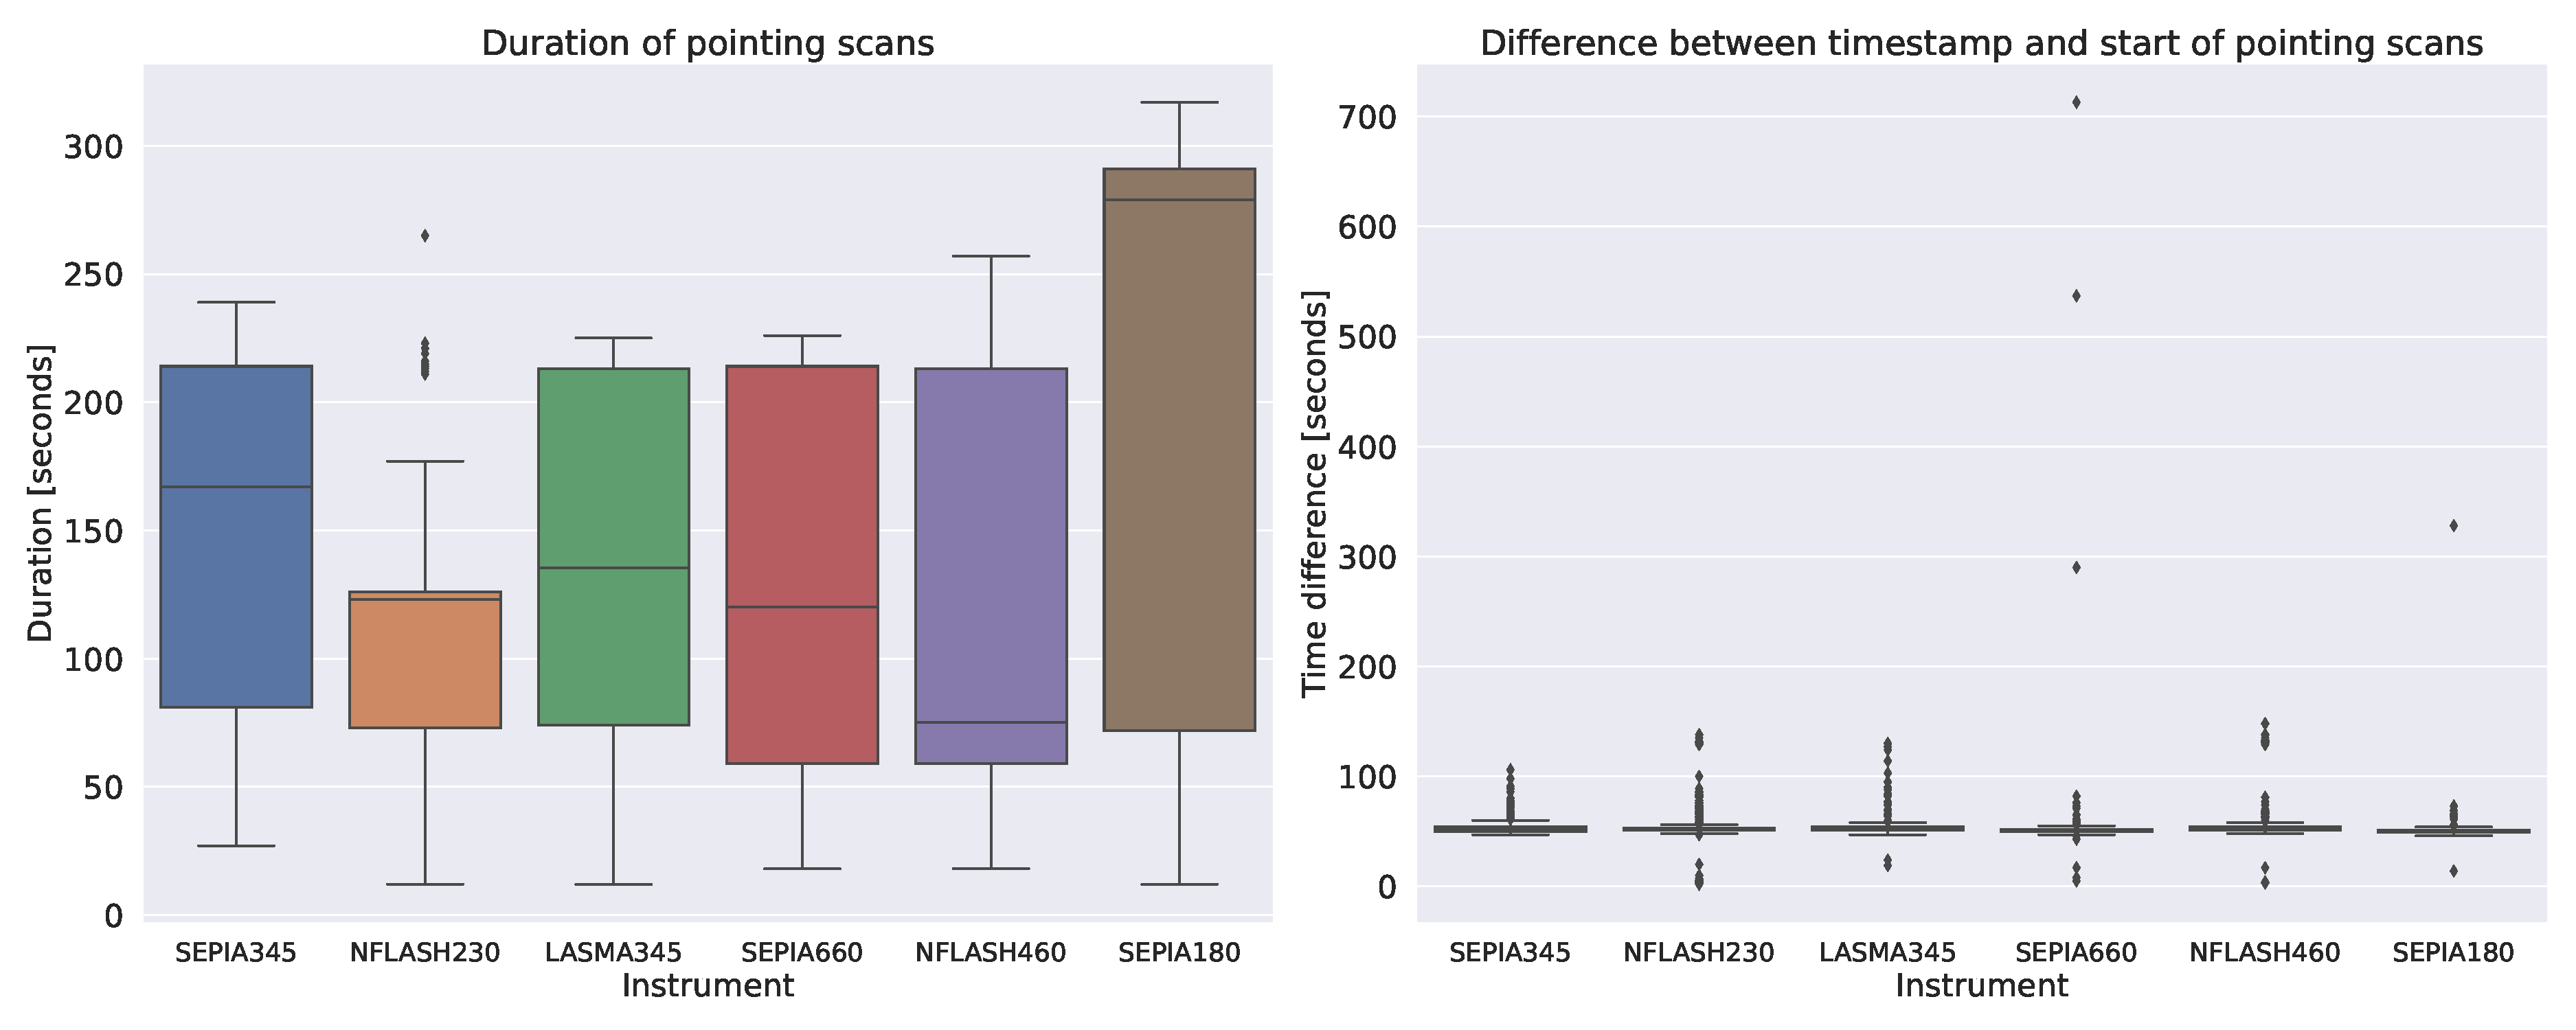
\includegraphics[width=1.1\textwidth]{Tiltmeter plots/scan_duration_distribution_rx.pdf}
    \caption{Box plot of the duration of scans, and the time difference between the timestamp of a scan and the actual start of it.}
    \label{fig:scan_times_box}
\end{figure}

\begin{figure}[H]
    \centering
    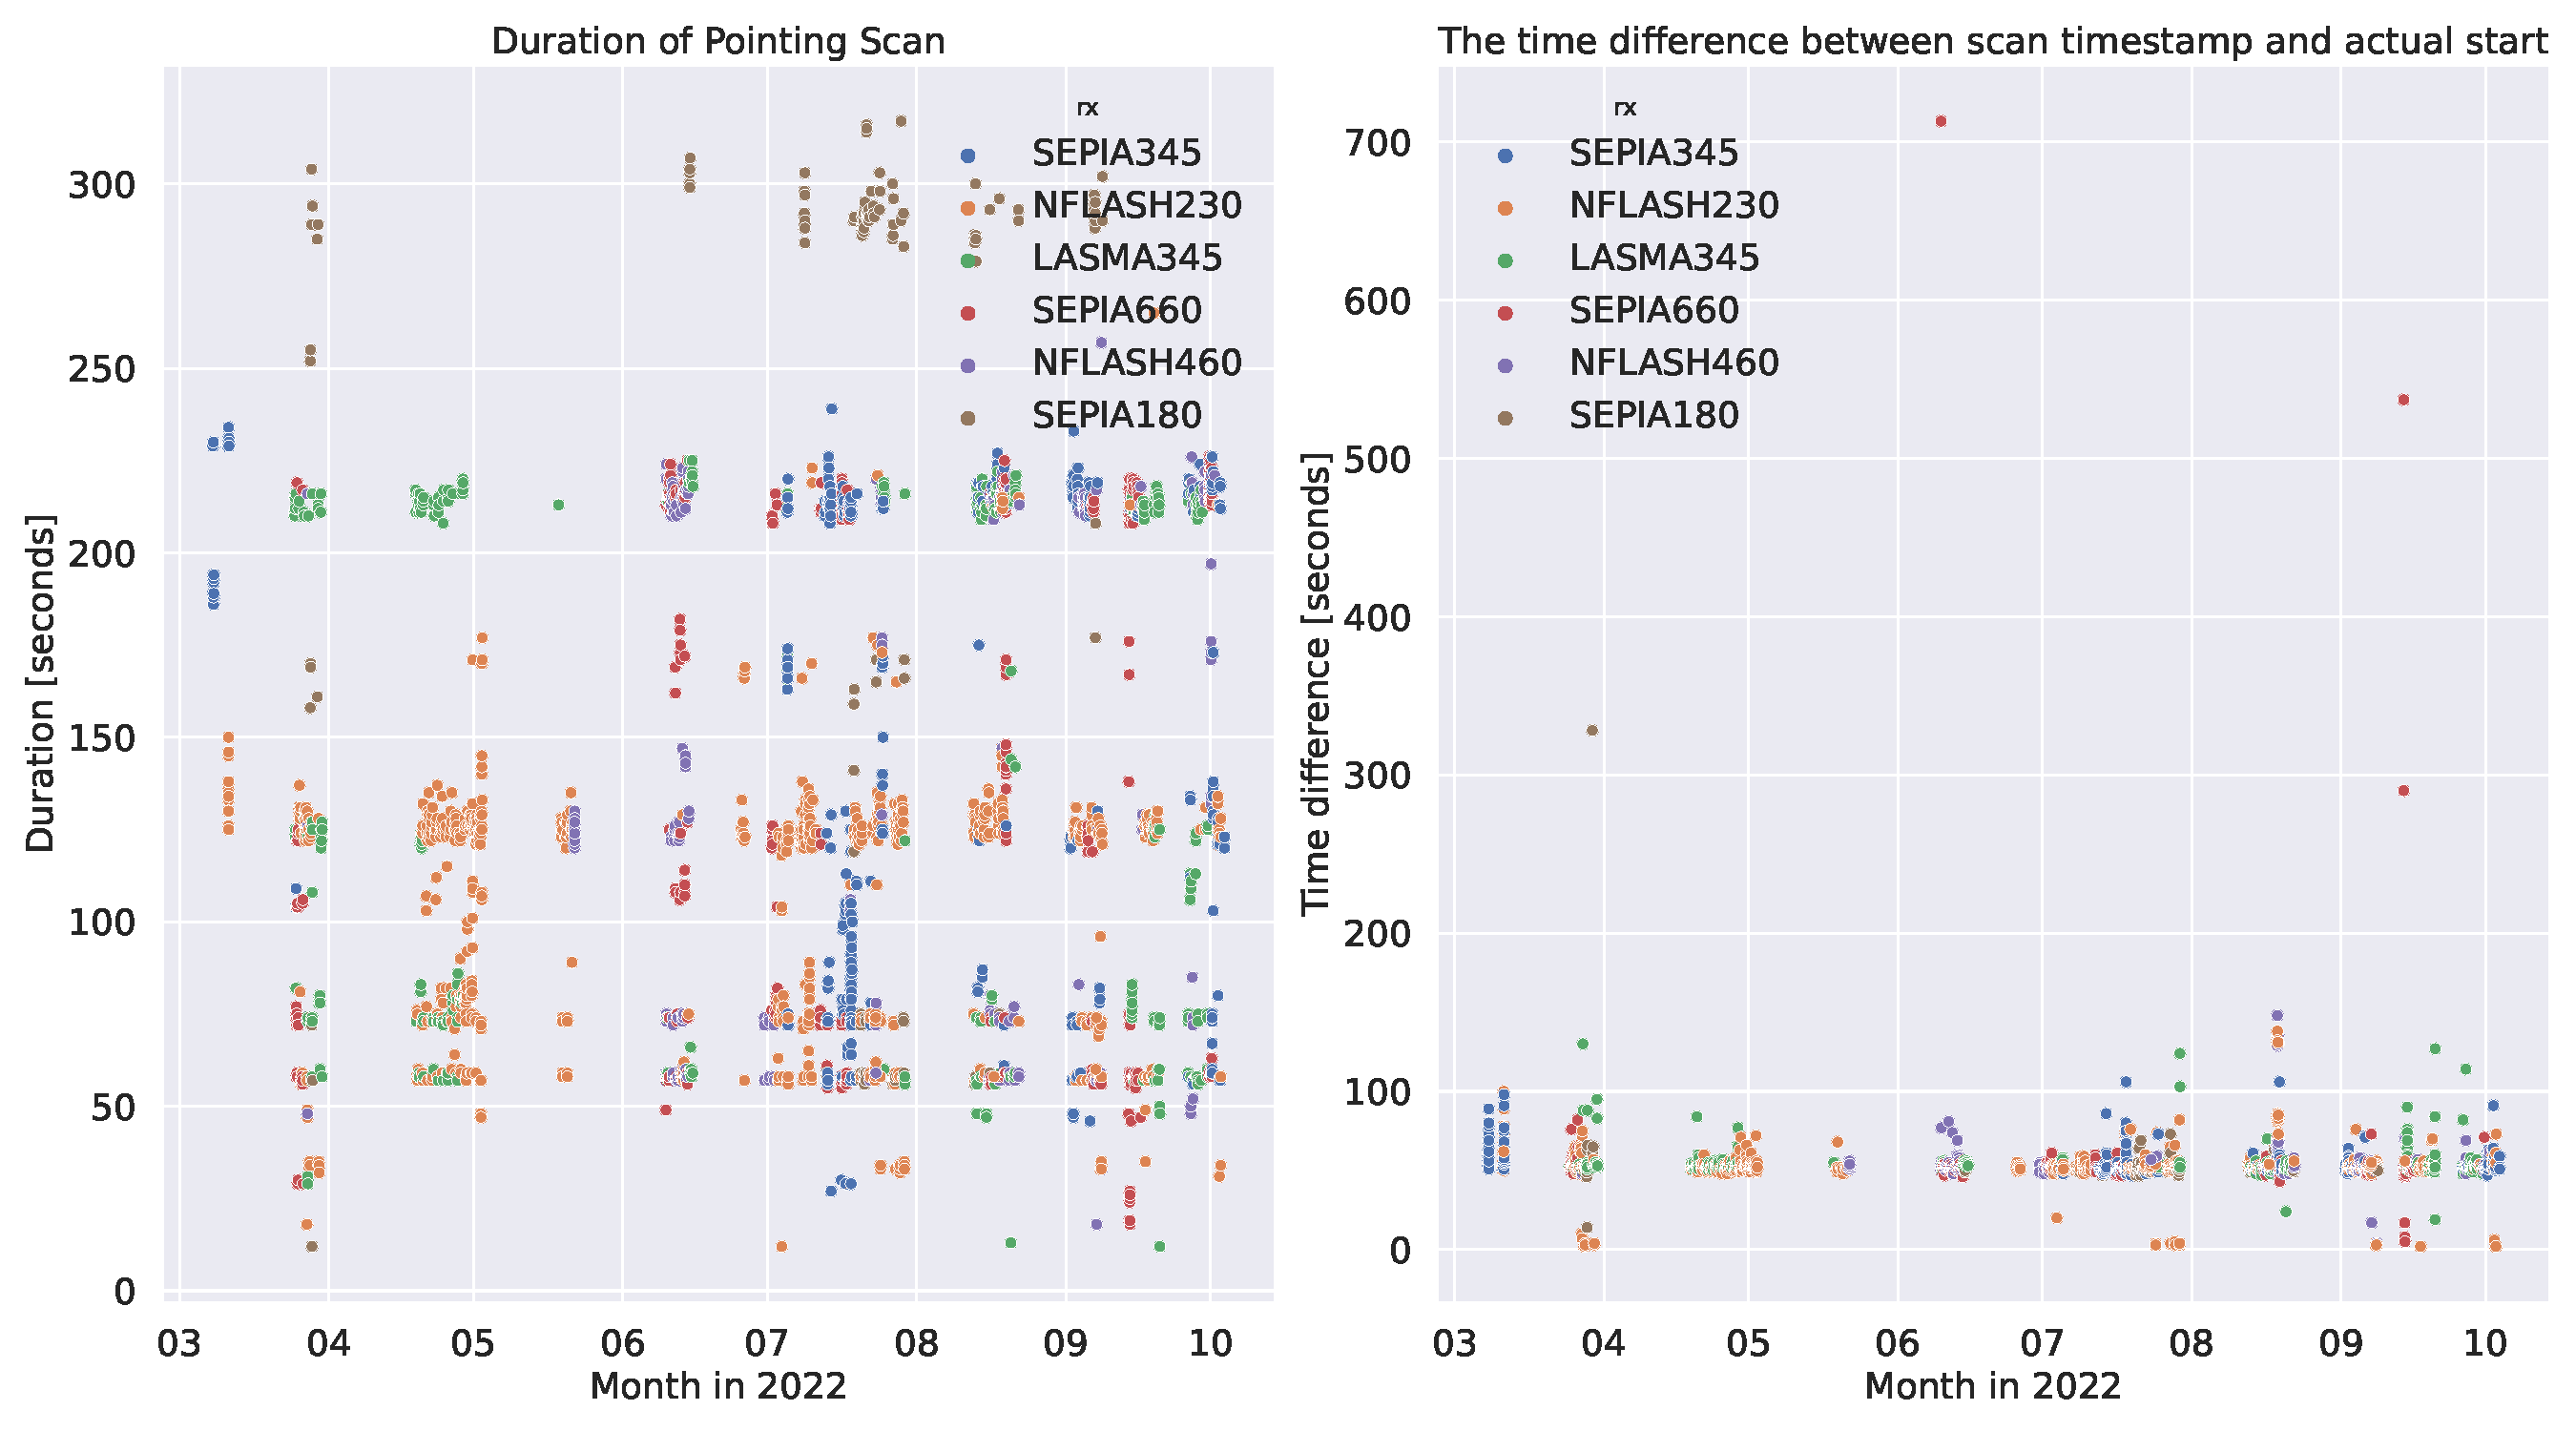
\includegraphics[width=1.1\textwidth]{Tiltmeter plots/scan_duration_distribution_date.pdf}
    \caption{Scatter plot of the duration of scans, and the time difference between the timestamp of a scan and the actual start of it.}
    \label{fig:scan_times_date}
\end{figure}




\section{Feature Engineering}\label{sec:feature_engineering}
There are two main features engineered for this project; features that represent the system during a pointing scan and features that represent changes since the last correction. 
The idea behind this is simple. The correction used during a pointing scan represents the ideal correction for the system during the previous pointing scan.
As there are a lot of factors and complex relationships, and we do not have large amounts of training data, it might be easier for the model to learn 
how these changes affect the pointing rather than learning all the relationships.

Table \textcolor{red}{ref table with a list of variables with median value} show all features.

% \textcolor{red}{Put this in feature engineering section}
% \begin{align}
%     \Delta \textit{Az}_\textit{wind} = \textit{Az}_\textit{pointing} - \textit{Az}_\textit{wind}
% \end{align}

% For the turbulence, a simple model is used
% \begin{align}
% v_\textit{wind} = \sigma_\textit{wind}^2
% \end{align}

\paragraph{Median values}
The median value of variables during a pointing scan is the most used feature.

\paragraph{Sum of all change}
To capture systematic error in pointing due to the telescope moving back and forth in azimuth and elevation,
we sum over the positive and negative changes in these variables.

Given the time of the last pointing correction $t_1$ and the start of a pointing scan $t_2$, the sum over the positive changes in a variable $x_i$ is given by
\begin{equation}\label{eq:positive_int}
    X = \sum_{i=t_1+1}^{t_2} \max(0, x_i-x_{i-1})
\end{equation}

Similarly, the sum of negative changes in a variable is
\begin{equation}\label{eq:negative_int}
    X = \sum_{i=t_1+1}^{t_2} \min(0, x_i-x_{i-1})
\end{equation}

We make these features with azimuth and elevation.

\paragraph{Change since the last correction}
This feature is self-explanatory and is just the change in a variable since the pointing was corrected.
\begin{equation}
    \Delta x = x_{t_2} - x_{t_1}
\end{equation}

In order to make this feature more robust against noisy data,
we instead consider the change in the median for a time interval around the last correction $t_1$ and the start of a pointing scan $t_2$

\begin{equation}
    \Delta x = \textit{median}(x_{t_2}, x_{t_2 - 1}, \dots, x_{t_2- p}) - \textit{median}(x_{t_1}, x_{t_1 + 1}, \dots, x_{t_1 + p}),
\end{equation}
where $p$ is the number of data points needed to cover a period of $P$ minutes, given by $p = P \cdot frequency$. The unit of frequency is data points per minute, found in Table \ref{tab:data_frequency}.

\paragraph{Max change in time interval}
In case the speed of the temperature change affects the deformation of the telescope's structure, we find the maximum temperature change in a given time interval since the last pointing correction.

\begin{equation}
    X = \max (x_{t_1+p} - x_{t_1}, x_{t_1+p} - x_{t_1}, \dots, x_{t_2} - x_{t_2-p}),
\end{equation}


\paragraph{Position of the sun}
Observers at the telescope report that the sun is affecting the pointing.
It is most drastically affected when the sun sets or rises, likely due to rapid temperature change leading to deformation in the telescope structure.
We also think the sun's position affects the pointing.
For instance, if the sun is shining on the left side of the telescope, it will affect the pointing differently than if it is on the right side.
Obtaining the sun's position for the telescope's location is done using the python module PyEphem \cite{ephem}.

Using the azimuth angle of the sun and the telescope, we can calculate the position of the sun with respect to the pointing with
\begin{equation}\label{eq:sun_az_diff}
    \Delta \textit{Az}_\odot = \textit{Az}_{\textit{t}} - \textit{Az}_\odot
\end{equation}
This will result in values outside the $[-180^\circ,180^\circ]$. An example is if $Az_\odot=179^\circ$ and $Az_t = -179^\circ$.
The calculation in equation \eqref{eq:sun_az_diff} yield $-179^\circ-179^\circ=-358^\circ$,
which corresponds to the sun being $358^\circ$ to the right of the telescope, while it ideally should be $2^\circ$ to the left.
Therefore, we adjust the values accordingly
%Write equations where \Delta Az_\odot above 180 is -= 360 and under 180 is += 360
\begin{align}
    \Delta Az_\odot = Az_\odot +360^\circ, \; \text{for} \; \Delta Az_\odot < 180^\circ\\
    \Delta Az_\odot = Az_\odot -360^\circ, \; \text{for} \; \Delta Az_\odot > 180^\circ
\end{align}

Here, the interval of the difference in azimuth is fixed to the interval $(-180^\circ,180^\circ)$,
where $0^\circ$ means the telescope is pointing towards the sun in the azimuth direction.
$\Delta \textit{Az}_\odot = 90^\circ$ corresponds to the sun being direct to the left of the pointing direction. \\

Another measure tested is the total angle between the pointing and the sun's position. We calculate this using the following formula
\begin{equation}
    \theta = \cos \textit{Az}_t \cdot \cos \textit{El}_t\cdot \cos \textit{Az}_\odot \cdot \cos \textit{El}_\odot + \sin \textit{Az}_t \cdot \cos \textit{El}_t\cdot \sin \textit{Az}_\odot \cdot \cos \textit{El}_\odot + \sin \textit{El}_t \cdot \sin \textit{El}_\odot
\end{equation}

\subsection{List of features}
\textcolor{red}{add a list of all features for different calculations here}

% \begin{table}[H]
%     \centering
%     \caption{Example from the dataset of the observed pointing offsets and the corrections applied during the pointing scan.}
%     \label{tab:offset_and_correction}
%     \begin{tabular}{ccccc}
%     \toprule
%     $i$ &  $\delta_{az}$ &  $\delta_{el}$ &  $ca$ & $ie$  \\
%     \midrule
%     1 & 1.2 & 0.1 & 2.1 &  1.7 \\
%     2 &     0.0 & 0.5 & 3.3 &  1.6 \\
%     3 &    -1.1 & 0.0 & 3.3 &  1.6 \\
%     4 &     0.6 & 0.7 & 2.2 &  1.6 \\
%     5 &     0.9 & 1.4 & 2.2 &  1.6 \\
%     6 &     1.0 & 1.1 & 2.2 &  1.6 \\
%     7 &    -0.9 & 1.2 & 3.1 &  0.5 \\
%     8 &     0.5 & 1.5 & 2.2 & -0.7 \\
%     9 &    -0.3 & 0.4 & 2.2 & -0.7 \\
%     \bottomrule
%     \end{tabular}
% \end{table}


% \begin{table}[H]
%     \centering
%     \caption{Table of transformed pointing offsets and corrections according to equations \eqref{eq:ca_tilde}, \eqref{eq:ie_tilde}, \eqref{eq:off_az_tilde}, and \eqref{eq:off_el_tilde}.}
%     \label{tab:tranform_offsets}
% \begin{tabular}{ccccc}
% \toprule
% $i$ & $\Tilde{\delta}_{az}$ &  $\Tilde{\delta}_{el}$ &  $\Tilde{ca}$ &  $\Tilde{ie}$ \\
% \midrule
% 0 &       1.2 &       0.1 &       2.1 &       1.7 \\
% 1 &       0.0 &       0.5 &       3.3 &       1.6 \\
% 2 &      -1.1 &      -0.5 &       3.3 &       1.1 \\
% 3 &       0.7 &       0.7 &       2.2 &       1.6 \\
% 4 &       0.2 &       0.7 &       2.8 &       0.9 \\
% 5 &       0.1 &      -0.3 &       3.1 &       0.2 \\
% 6 &      -1.0 &       1.3 &       3.2 &       0.5 \\
% 7 &       0.5 &       1.4 &       2.2 &      -0.7 \\
% 8 &      -0.8 &      -1.1 &       2.7 &      -2.2 \\
% \bottomrule
% \end{tabular}
% \end{table}


\section{Machine Learning Experiments}\label{sec:ml_exp}
In this section, we will provide an overview of two machine learning experiments pertinent to the two research questions. \textcolor{red}{refer to section with research qs}
The first experiment aims to investigate the effectiveness of neural networks in developing a pointing model that could replace the current linear model, which is created through linear regression.
It explores the feasibility of a more sophisticated model in terms of pointing accuracy.
The second experiment aims to examine the effectiveness of an XGBoost model in predicting pointing scan offsets to enhance the pointing accuracy.
The primary objective of this experiment is to assess whether the proposed model can outperform the current model in terms of pointing accuracy.

\subsection{Experiment 1: Pointing Model using Neural Networks}
This experiment uses the raw dataset containing input coordinates, $Az_{\text{input}}$ and $El_{\text{input}}$ respectively, and corresponding true observed values $Az_{\text{observed}}$ and $El_{\text{observed}}$.

The goal is to find a model $f$ such that
\begin{equation}
    f(X) \approx (\delta_{\text{Az}}, \delta_{\text{El}}) = (Az_{\text{observed}}-Az_{\text{input}}, El_{\text{observed}}-El_{\text{input}})
\end{equation}

We split the data into a train, validation, and test set.
The last $15\%$ of the data, which we sorted by date, is used for testing.
We use the remaining $85\%$ of the data for training and validation and split this set into $20\%$ for training and $80\%$ for validation.
This results in $\approx 76\%$ and $\approx 24\%$ of the total dataset used for training and validation.

\subsubsection{Feature Selection}
Selecting the right features is essential in improving the pointing model's accuracy.
This model uses two types of features: geometrical and harmonic terms already part of the current linear base model and new features extracted from the telescope's database.
We identified relevant features by calculating Pearson's and Spearman's rank correlation to the offsets for all features.
We analyzed the correlation of the geometrical terms, and harmonic terms using sine and cosine functions of azimuth and elevation up to the fifth order.
Then, we chose the terms with the strongest correlation to the model and used them in all models.
We made a list of the features we extracted from the database that showed a correlation equal to or greater than 0.1.
During model training, we randomly selected a subset of 2 to 19 features from this list and used them to train the model.

\subsubsection{Model Architecture}
This experiment utilized four different model architectures.
The first architecture involved feeding all input data into one, two, or three hidden layers.
The other three architectures incorporated machine learning techniques by separating the geometrical and harmonic terms of the input data from the other features and processing them using distinct architectures.
With these approaches, we intend to keep the current model's simplicity and performance while incorporating new features.

The following are the four different architectures:
\begin{enumerate}
    \item \textbf{Regular Neural Network:} All features are passed through the same layers, all with a nonlinear activation function.
    See Figure \ref{subfig:regular}
    \item \textbf{Neural Network with Separated Features 1:} This architecture separates the input features into two groups: geometric and harmonic features, and the rest of the features.
    The geometric and harmonic features are connected directly to the linear output layer, while we pass the remaining features through layers with nonlinear activation functions.
    See Figure \ref{subfig:comb_sep1}
    \item \textbf{Neural Network with Separated Features 2:} This architecture is similar to the previous architecture,
    but we feed the geometric and harmonic features through an additional layer of nonlinear activation function before connecting them to the output layer.
    See Figure \ref{subfig:comb_sep2}
    \item \textbf{Neural Network with Separated Features 3:} This architecture combines the previous two architectures by passing the regular features through a few hidden layers with nonlinear activation functions before concatenating them with the geometric and harmonic features.
    We then pass the combined features through a final layer before connecting them to the output layer.
    See Figure \ref{subfig:comb_sep3}
\end{enumerate}
These are visualized in Figure \ref{fig:nn_architecture}.

\begin{figure}[H]
    \centering
    \begin{subfigure}[t]{0.49\textwidth}
        \centering
        % NEURAL NETWORK no text - large
\begin{tikzpicture}[x=2.3cm,y=1.0cm]
  \message{^^JNeural network large}
  \readlist\Nnod{3,4,4,2} % array of number of nodes per layer
  
  \message{^^J  Layer}
  \foreachitem \N \in \Nnod{ % loop over layers
    \def\lay{\Ncnt} % alias of index of current layer
    \pgfmathsetmacro\prev{int(\Ncnt-1)} % number of previous layer
    \message{\lay,}
    \foreach \i [evaluate={\y=\N/2-\i; \x=\lay*0.8; \n=\nstyle;
                           \nprev=int(\prev<\Nnodlen?min(2,\prev):3);}] in {1,...,\N}{ % loop over nodes
      
      % NODES
      %\node[node \n,outer sep=0.6,minimum size=18] (N\lay-\i) at (\x,\y) {};
      \coordinate (N\lay-\i) at (\x,\y);
      
      % CONNECTIONS
      \ifnum\lay>1 % connect to previous layer
        \foreach \j in {1,...,\Nnod[\prev]}{ % loop over nodes in previous layer
          \draw[connect,white,line width=1.2] (N\prev-\j) -- (N\lay-\i);
          \draw[connect] (N\prev-\j) -- (N\lay-\i);
          %\draw[connect] (N\prev-\j.0) -- (N\lay-\i.180); % connect to left
          \node[node \nprev,minimum size=18] at (N\prev-\j) {}; % draw node over lines
        }
        \ifnum \lay=\Nnodlen % draw last node over lines
          \node[node \n,minimum size=18] at (N\lay-\i) {};
        \fi
      \fi % else: nothing to connect first layer
      
    }
  }
  
\end{tikzpicture}
        \caption{\textbf{Regular neural network:}
        This is the standard neural network architecture without any feature separation.
        All features are connected to the same layers.}
        \label{subfig:regular}
    \end{subfigure}
    \hfill
   \begin{subfigure}[t]{0.49\textwidth}
       \centering
       \begin{tikzpicture}[x=2.3cm,y=2.0cm]
  \message{^^JNeural network large}
  \readlist\Nnod{3,2} % array of number of nodes per layer
  \readlist\Nnodtwo{2,3,3,2}
  \message{^^J  Layer}
  \foreachitem \N \in \Nnod{ % loop over layers
    \def\lay{\Ncnt} % alias of index of current layer
    \pgfmathsetmacro\prev{int(\Ncnt-1)} % number of previous layer
    \message{\lay,}
    \foreach \i [evaluate={\y=\N/4-\i*0.5; \x=\lay*0.8+1.6; \n=\nstyle;
                           \nprev=int(\prev<\Nnodlen?min(2,\prev):3);}] in {1,...,\N}{ % loop over nodes
      
      % NODES
      %\node[node \n,outer sep=0.6,minimum size=18] (N\lay-\i) at (\x,\y) {};
      \ifnum \lay<\Nnodlen % draw last node over lines
        \coordinate (N\lay-\i) at (\x,\y);
      \else
        \coordinate (N\lay-\i) at (\x,\y-0.75);
      \fi
      % CONNECTIONS
      \ifnum\lay>1 % connect to previous layer
        \foreach \j in {1,...,\Nnod[\prev]}{ % loop over nodes in previous layer
          \draw[connect,white,line width=1.2] (N\prev-\j) -- (N\lay-\i);
          \draw[connect] (N\prev-\j) -- (N\lay-\i);
          %\draw[connect] (N\prev-\j.0) -- (N\lay-\i.180); % connect to left
          \node[node \nprev,minimum size=18] at (N\prev-\j) {}; % draw node over lines
        }
        \ifnum \lay=\Nnodlen % draw last node over lines
          \node[node \n,minimum size=18] at (N\lay-\i) {};
        \fi
      \fi % else: nothing to connect first layer
      
    }
  }

  \foreachitem \N \in \Nnodtwo{ % loop over layers
    \def\lay{\Ncnt} % alias of index of current layer
    \pgfmathsetmacro\prev{int(\Ncnt-1)} % number of previous layer
    \message{\lay,}
    \foreach \i [evaluate={\y=\N/4-\i*0.5-1.5; \x=\lay*0.8; \n=\nstyle;
                           \nprev=int(\prev<\Nnodtwolen?min(2,\prev):3);}] in {1,...,\N}{ % loop over nodes
      % NODES
      %\node[node \n,outer sep=0.6,minimum size=18] (N\lay-\i) at (\x,\y) {};
      \ifnum \lay<\Nnodtwolen % draw last node over lines
        \coordinate (M\lay-\i) at (\x,\y);
      \else
        \coordinate (M\lay-\i) at (\x,\y+0.75);
      \fi
      % CONNECTIONS
      \ifnum\lay>1 % connect to previous layer
        \foreach \j in {1,...,\Nnodtwo[\prev]}{ % loop over nodes in previous layer
          \draw[connect,white,line width=1.2] (M\prev-\j) -- (M\lay-\i);
          \draw[connect] (M\prev-\j) -- (M\lay-\i);
          %\draw[connect] (N\prev-\j.0) -- (N\lay-\i.180); % connect to left
          \node[node \nprev,minimum size=18] at (M\prev-\j) {}; % draw node over lines
        }
        \ifnum \lay=\Nnodtwolen % draw last node over lines
          \node[node \n,minimum size=18] at (M\lay-\i) {};
        \fi
      \fi % else: nothing to connect first layer
      
    }
  }
  
\end{tikzpicture}
       \caption{\textbf{Neural network with separated features 1:}
       In this architecture, the geometric and harmonic features are separated from the other features and directly connected to the output layer without any nonlinear activation function.}
       \label{subfig:comb_sep1}
\end{subfigure}
\\~\\
    \begin{subfigure}[t]{0.49\textwidth}
        \centering
        \begin{tikzpicture}[x=2.3cm,y=2.0cm]
  \message{^^JNeural network large}
  \readlist\Nnod{3,3,2} % array of number of nodes per layer
  \readlist\Nnodtwo{2,3,3,2}
  \message{^^J  Layer}
  \foreachitem \N \in \Nnod{ % loop over layers
    \def\lay{\Ncnt} % alias of index of current layer
    \pgfmathsetmacro\prev{int(\Ncnt-1)} % number of previous layer
    \message{\lay,}
    \foreach \i [evaluate={\y=\N/4-\i*0.5; \x=\lay*0.8+0.8; \n=\nstyle;
                           \nprev=int(\prev<\Nnodlen?min(2,\prev):3);}] in {1,...,\N}{ % loop over nodes
      
      % NODES
      %\node[node \n,outer sep=0.6,minimum size=18] (N\lay-\i) at (\x,\y) {};
      \ifnum \lay<\Nnodlen % draw last node over lines
        \coordinate (N\lay-\i) at (\x,\y);
      \else
        \coordinate (N\lay-\i) at (\x,\y-0.75);
      \fi
      % CONNECTIONS
      \ifnum\lay>1 % connect to previous layer
        \foreach \j in {1,...,\Nnod[\prev]}{ % loop over nodes in previous layer
          \draw[connect,white,line width=1.2] (N\prev-\j) -- (N\lay-\i);
          \draw[connect] (N\prev-\j) -- (N\lay-\i);
          %\draw[connect] (N\prev-\j.0) -- (N\lay-\i.180); % connect to left
          \node[node \nprev,minimum size=18] at (N\prev-\j) {}; % draw node over lines
        }
        \ifnum \lay=\Nnodlen % draw last node over lines
          \node[node \n,minimum size=18] at (N\lay-\i) {};
        \fi
      \fi % else: nothing to connect first layer
      
    }
  }
  \node[shift = {(-1.5,0)}] at (N2-2){
    $\begin{aligned}
      \text{Geom}&\text{etric}\\
      +&\\
      \text{Harm}&\text{onics}
    \end{aligned}$
  };
  \node[shift = {(-1.5,-0.85)}] at (N2-2){Nonlinear};
  \foreachitem \N \in \Nnodtwo{ % loop over layers
    \def\lay{\Ncnt} % alias of index of current layer
    \pgfmathsetmacro\prev{int(\Ncnt-1)} % number of previous layer
    \message{\lay,}
    \foreach \i [evaluate={\y=\N/4-\i*0.5-1.5; \x=\lay*0.8; \n=\nstyle;
                           \nprev=int(\prev<\Nnodtwolen?min(2,\prev):3);}] in {1,...,\N}{ % loop over nodes
      % NODES
      %\node[node \n,outer sep=0.6,minimum size=18] (N\lay-\i) at (\x,\y) {};
      \ifnum \lay<\Nnodtwolen % draw last node over lines
        \coordinate (M\lay-\i) at (\x,\y);
      \else
        \coordinate (M\lay-\i) at (\x,\y+0.75);
      \fi
      % CONNECTIONS
      \ifnum\lay>1 % connect to previous layer
        \foreach \j in {1,...,\Nnodtwo[\prev]}{ % loop over nodes in previous layer
          \draw[connect,white,line width=1.2] (M\prev-\j) -- (M\lay-\i);
          \draw[connect] (M\prev-\j) -- (M\lay-\i);
          %\draw[connect] (N\prev-\j.0) -- (N\lay-\i.180); % connect to left
          \node[node \nprev,minimum size=18] at (M\prev-\j) {}; % draw node over lines
        }
        \ifnum \lay=\Nnodtwolen % draw last node over lines
          \node[node \n,minimum size=18] at (M\lay-\i) {};
        \fi
      \fi % else: nothing to connect first layer
      
    }
  }
  
\end{tikzpicture}
        \caption{\textbf{Neural network with separated features 2}:
        Similar to the previous architecture, the geometric and harmonic features are separated from the other features.
        However, they are also processed by a nonlinear activation function before being connected to the output layer.}
        \label{subfig:comb_sep2}
    \end{subfigure}
    \hfill
       \begin{subfigure}[t]{0.49\textwidth}
        \centering
        \begin{tikzpicture}[x=2.3cm,y=2.0cm]
  \message{^^JNeural network large}
  \readlist\Nnod{3,3,2} % array of number of nodes per layer
  \readlist\Nnodtwo{2,3,3,2}
  \message{^^J  Layer}
  \foreachitem \N \in \Nnod{ % loop over layers
    \def\lay{\Ncnt} % alias of index of current layer
    \pgfmathsetmacro\prev{int(\Ncnt-1)} % number of previous layer
    \message{\lay,}
    \foreach \i [evaluate={\y=\N/4-\i*0.5; \x=\lay*0.8+0.8; \n=\nstyle;
                           \nprev=int(\prev<\Nnodlen?min(2,\prev):3);}] in {1,...,\N}{ % loop over nodes
      
      % NODES
      %\node[node \n,outer sep=0.6,minimum size=18] (N\lay-\i) at (\x,\y) {};
      \ifnum \lay<\Nnodlen % draw last node over lines
        \coordinate (N\lay-\i) at (\x,\y);
      \else
        \coordinate (N\lay-\i) at (\x,\y-0.75);
      \fi
      % CONNECTIONS
      \ifnum\lay>1 % connect to previous layer
        \foreach \j in {1,...,\Nnod[\prev]}{ % loop over nodes in previous layer
          \draw[connect,white,line width=1.2] (N\prev-\j) -- (N\lay-\i);
          \draw[connect] (N\prev-\j) -- (N\lay-\i);
          %\draw[connect] (N\prev-\j.0) -- (N\lay-\i.180); % connect to left
          \node[node \nprev,minimum size=18] at (N\prev-\j) {}; % draw node over lines
        }
        \ifnum \lay=\Nnodlen % draw last node over lines
          \node[node \n,minimum size=18] at (N\lay-\i) {};
        \fi
      \fi % else: nothing to connect first layer
      
    }
  }

  \foreachitem \N \in \Nnodtwo{ % loop over layers
    \def\lay{\Ncnt} % alias of index of current layer
    \pgfmathsetmacro\prev{int(\Ncnt-1)} % number of previous layer
    \message{\lay,}
    \foreach \i [evaluate={\y=\N/4-\i*0.5-1.5; \x=\lay*0.8; \n=\nstyle;
                           \nprev=int(\prev<\Nnodtwolen?min(2,\prev):3);}] in {1,...,\N}{ % loop over nodes
      % NODES
      %\node[node \n,outer sep=0.6,minimum size=18] (N\lay-\i) at (\x,\y) {};
      \ifnum \lay<\Nnodtwolen % draw last node over lines
        \coordinate (M\lay-\i) at (\x,\y);
      \else
        \coordinate (M\lay-\i) at (\x,\y+0.75);
      \fi
      % CONNECTIONS
      \ifnum\lay>1 % connect to previous layer
        \foreach \j in {1,...,\Nnodtwo[\prev]}{ % loop over nodes in previous layer
          \draw[connect,white,line width=1.2] (M\prev-\j) -- (M\lay-\i);
          \draw[connect] (M\prev-\j) -- (M\lay-\i);
          %\draw[connect] (N\prev-\j.0) -- (N\lay-\i.180); % connect to left
          \node[node \nprev,minimum size=18] at (M\prev-\j) {}; % draw node over lines
        }
        \ifnum \lay=\Nnodtwolen % draw last node over lines
          \node[node \n,minimum size=18] at (M\lay-\i) {};
        \fi
      \fi % else: nothing to connect first layer
      
    }
  }

  \foreachitem \N \in \Nnod{ % loop over layers
    \def\lay{\Ncnt} % alias of index of current layer
    \pgfmathsetmacro\prev{int(\Ncnt-1)} % number of previous layer
    \message{\lay,}
    \foreach \i [evaluate={\y=\N-\i*0.5; \x=\lay; \n=\nstyle;
                           \nprev=int(\prev<\Nnodlen?min(2,\prev):3);}] in {1,...,\N}{ % loop over nodes
      
      % CONNECTIONS
      \ifnum\lay=2 % connect to previous layer
        \foreach \j in {1,...,\Nnod[\prev]}{ % loop over nodes in previous layer
          \draw[connect,white,line width=1.2] (M3-\j) -- (N\lay-\i);
          \draw[connect] (M3-\j) -- (N\lay-\i);
          %\draw[connect] (N\prev-\j.0) -- (N\lay-\i.180); % connect to left
          \message{^^J Nprev \nprev}
          \node[node 2,minimum size=18] at (M3-\j) {}; % draw node over lines
          \node[node 2,minimum size=18] at (N\lay-\j) {}; % draw node over lines
        }
      \fi % else: nothing to connect first layer
      
    }
  }

  \foreachitem \N \in \Nnodtwo{ % loop over layers
    \def\lay{\Ncnt} % alias of index of current layer
    \pgfmathsetmacro\prev{int(\Ncnt-1)} % number of previous layer
    \message{\lay,}
    \foreach \i [evaluate={\y=\N/4-\i*0.5; \x=\lay+2; \n=\nstyle;
                           \nprev=int(\prev<\Nnodtwolen?min(2,\prev):3);}] in {1,...,\N}{ % loop over nodes
      % NODES
      %\node[node \n,outer sep=0.6,minimum size=18] (N\lay-\i) at (\x,\y) {};
      \ifnum\lay=3 % connect to previous layer
        \foreach \j in {1,...,\Nnodtwo[\prev]}{ % loop over nodes in previous layer
          \message{^^J \lay Here (N1-\j) {l\lay}}
          \draw[connect,white,line width=1.2] (N1-\j) -- (M\lay-\i);
          \draw[connect] (N1-\j) -- (M\lay-\i);
          %\draw[connect] (N\prev-\j.0) -- (N\lay-\i.180); % connect to left
          \node[node 1,minimum size=18] at (N1-\j) {}; % draw node over lines
          \node[node 2,minimum size=18] at (M\lay-\j) {}; % draw node over lines
          
        }

      \fi % else: nothing to connect first layer
      
    }
  }



\end{tikzpicture}
        \caption{\textbf{Neural network with separated features 3:}
        In this architecture, we concatenate the processed regular features to the geometric and harmonic features before being connected to the output layer.}
        \label{subfig:comb_sep3}
    \end{subfigure}
     \caption{These architectures were used to train a base pointing model on raw data.}
     \label{fig:nn_architecture}
\end{figure}

The hyperparameters for the neural networks were randomly sampled from different distributions, as presented in Table \ref{tab:nn_hyperparameters}.
Some parameters were consistent across all models, such as the Adam optimization algorithm and the mean squared error loss function.
In total, \textcolor{red}{input the number of fitted NNs here} networks of each architecture are trained for $300$ epochs.
We pick the model from the epoch with the best performance on the validation set.
\begin{table}[H]
    \centering
    \caption{This table presents a list of parameters we sampled during hyperparameter tuning for the base pointing model. The table includes names, the distribution we sampled from, and corresponding ranges.}
    \begin{tabular}{lcc}
    \hline
    \textbf{Name} & \textbf{Distribution Type} & \textbf{Range} \\ \hline
    hidden layers & uniform integer & [$1$,$3$] \\
    hidden layer size & uniform integer & [$20$, $120$] \\
    learning rate & uniform & [$0.001$, $0.02$] \\
    batch size & uniform integer & [$32$, $512$] \\
    activation & categorical & [gelu, tanh] \\ \hline
    \end{tabular}
    \label{tab:nn_hyperparameters}
    \end{table}

\subsubsection{Loss Function and Model Evaluation}
To evaluate the performance of the models, we used the root mean squared (RMS), measured in arcseconds, on the test set.
We calculate the RMS as follows:
\begin{equation}
    \text{RMS} = \sqrt{ \frac{1}{N} \sum_{i=1}^N \left( (\tilde{\delta}_{Az,i} - \delta_{Az,i})^2 + (\tilde{\delta}_{El,i} - \delta_{El,i})^2 \right)},
\end{equation}
where $\tilde{\delta}_{Az}$ and $\tilde{\delta}_{El}$ are the predicted offsets, while $\delta_{Az}$ and $\delta_{El}$ are the true values.
$N$ is the number of observations in the test set.

This RMS is used to compare the performance of the models.
It will also be compared with a benchmark linear regression model to see if a machine learning approach offers any improvements.

\subsection{Experiment 2: Pointing Correction Model}
This experiment aims to improve the accuracy of the existing pointing model by training XGBoost models to predict offsets obtained from pointing scans.
To accomplish this, we utilized two different datasets, which we processed using the cleaning outlined in section \ref{sec:cleaning_pt_scan}.
The difference between these datasets is that one contains the scans from all instruments, while the other only contains the scans from NFLASH230.
By training our models on these datasets, we aim to reduce the pointing offset and improve the accuracy of the pointing.
In addition, we varied the way we split the datasets for training and testing.
We considered two cases:

\begin{itemize}
    \item \textbf{Case 1:} The dataset is sorted by date and split into six equal-sized folds.
    We consider each of the folds one by one.
    For each of these folds, we use the last $1/6$th of the data as a test set and the remaining $5/6$th as training and validation.
    \item \textbf{Case 2:} The dataset is sorted by date and split into six equal-sized folds.
    We used $5/6$ of the data for training and validation and the remaining for testing.
    We repeated this process six times, using each fold for testing once.
\end{itemize}

Figure \ref{fig:datasplit_cases} illustrates the two cases.
In both cases, we trained and validated the model on $5/6$ of the data and tested on the last $1/6$.
The difference is the amount of data used for training, which can indicate whether models trained on shorter or longer periods perform better.
Using longer period, and thus more data, can help the model find complex relations.
However, a smaller period may be better for learning relations that change over time, as we would expect less variation in a shorter period.

We also split the training and validation data such that scans from a given day only can be either in the training or validation set, not both.
When splitting the data, we used $35\%$ of the days for validation and $65\%$ for training.
This does not amount to precisely the same percentage of scans for the given split, but something close to it nonetheless.


\begin{figure}[H]
    \centering
    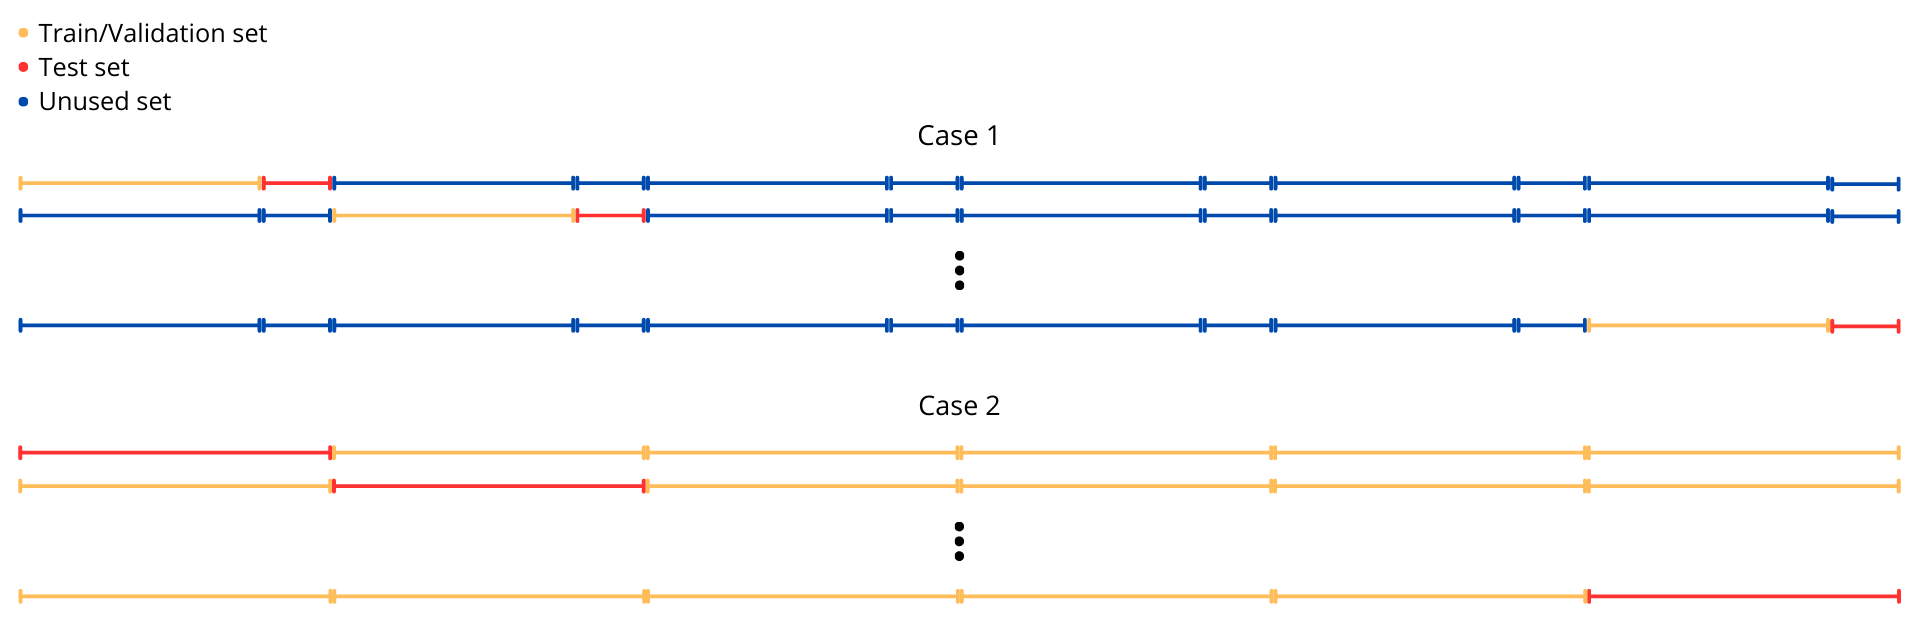
\includegraphics[width=0.98\textwidth]{Canva/datasplits.png}
    \caption{This figure shows two cross-validation cases: the orange region represents the train and validation set, the red region represents the test set, and the blue region is unused for evaluation.
    In \textbf{Case 1}, the dataset is split into six equal-sized folds sorted by date.
    For the selected fold, we use the last part (colored red) for testing and the remaining part (colored orange) for training and validation.
    This process is repeated six times, once for each fold.
    In \textbf{Case 2}, the dataset is again split into six equal-sized folds sorted by date.
    However, we use one whole fold for testing this time and the remaining five for training and validation.
    This process is repeated six times, with each fold used exactly once for testing.}
    \label{fig:datasplit_cases}
\end{figure}




\subsubsection{Feature Selection}
We trained models using a range of features, specifically $k=[2,5,10,20,30,40,50]$ features.
We selected the $k$ features that had the greatest mutual information for each model with the target value.
This approach helps us identify the most important features to improve the model's performance. Selecting a subset of features can reduce the noise in the data. 
By selecting different numbers of features, we can explore the trade-off between model complexity and performance.\textcolor{red}{write and ref to mutual info in theory section}.

\subsubsection{Model Architecture}
We performed a Bayesian hyperparameter search for each model using the parameter space in Table \ref{tab:xgb_hyperparameters_pcorr}.
The search space includes eight hyperparameters that affect the model's complexity, such as the maximum depth of the trees, the regularization strength, and the learning rate.
We used a uniform or log-uniform distribution to sample each hyperparameter within a specific range.
We evaluated $200$ different combinations of hyperparameters (for each dataset, cross-validation case, target variable, and the number of features selected) to find the optimal values for each model.
The models were validated using the MSE, and we picked the model with the best performance on the validation set.


\begin{table}[H]
    \centering
    \caption{This table presents a list of parameters we sampled during hyperparameter tuning for the pointing correction model. The table includes names, sampled distributions, and corresponding ranges.}
    \begin{tabular}{lcc}
        \toprule
        \textbf{Parameter} & \textbf{Sample Distribution} & \textbf{Range} \\ \hline
        max depth & Uniform & [$1$, $5$] \\ 
        reg lambda & Uniform & [$0$, $1$] \\ 
        colsample bytree & Uniform & [$0.5$, $1$] \\ 
        n estimators & Uniform & [$20$, $500$] \\ 
        learning rate & Log-Uniform & [$10^{-5}$, $1$] \\ 
        subsample & Uniform & [$0.5$, $1$] \\ 
        gamma & Log-Uniform & [$10^{-5}$, $1$] \\ 
        min child weight & Uniform & [$1$, $10$] \\ 
        \bottomrule
    \end{tabular}
    \label{tab:xgb_hyperparameters_pcorr}
\end{table}



\subsubsection{Model Evaluation}
To evaluate the performance of the models, we calculated the RMS on each test fold and compared it to the current RMS of the telescope on the same data.
The RMS is calculated for azimuth and elevation separately since an XGBoost model only can predict one target.
For a fold $j$ and target either azimuth or elevation, we calculate the RMS by
\begin{equation}
    RMS_{\text{target},j} = \sqrt{\frac{1}{N_j}\sum_{i=1}^{N_j} (\tilde{\delta}_{\text{target},ji} - \delta_{\text{target},ji})^2},
\end{equation}
where $\tilde{\delta}_{\text{target},ji}$ is the predicted pointing offset and $\delta_{\text{target},ji}$ is the true pointing offset for the $i$th pointing scan in fold $j$.
$N_j$ is the number of pointing scans in fold $j$. 
We then computed the ratio $r_{RMS,j}$ of the model's RMS to the current RMS for each fold.
If the ratio is less than $1$, it indicates that the XGBoost model provides an improvement over the current performance of the telescope for a given fold.

To obtain an overall measure of the model's performance compared to the current performance of the telescope, we averaged the ratios $r_{RMS,j}$ over all six test folds
\begin{equation} \label{eq:mean_rms_compared}
    \bar{r}_{RMS} = \sum_{i=1}^6 \frac{RMS_{model,j}}{RMS_{current,j}}.
\end{equation}
This gives us an average ratio $\bar{r}_{RMS}$, which measures the improvement in performance provided by the XGBoost model.
If $\bar{r}_{RMS} < 1$, it indicates that the XGBoost model outperforms the current pointing correction method on average across all test folds.
By comparing the average ratio $\bar{r}_{RMS}$ for the two different cross-validation cases in Figure \ref{fig:datasplit_cases} and the selected number of features,
we can identify which models provide the best performance.
